\documentclass{article}
\linespread{1.3}
\usepackage[margin=50pt]{geometry}
\usepackage{amsmath, amsthm, amssymb, amsthm, tikz, fancyhdr, graphicx}
\pagestyle{fancy}
\renewcommand{\headrulewidth}{0pt}
\newcommand{\changefont}{\fontsize{15}{15}\selectfont}

\fancypagestyle{firstpageheader}
{
  \fancyhead[R]{\changefont Michael Huang \\ CFRM 420 \\ Homework 1}
}

\begin{document}

\thispagestyle{firstpageheader}

\section*{1.}
{\Large 

\subsection*{(a)}

To calculate the daily arithmetic returns, we take the adjusted stock prices for each day $n$ and simply calculate the daily returns like so: \\
$R(t_{n-1}, t_n) = \frac{{P_t}_n - P_t_{n-1}}{{P_t}_{n-1}}$ \\
Which we then plot.

\begin{figure}[h]
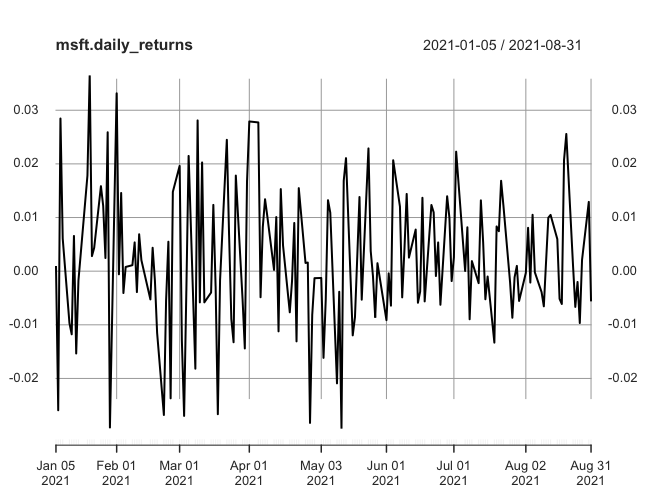
\includegraphics[width=500pt]{hw1_1a.png}}
\centering
\end{figure}

\subsection*{(b)}

To calculate the monthly log returns, we take each time period $n$ and evaluate like so: \\
$r(t_{n-1}, t_n) = \text{log}\frac{{P_t}_{n}}{{P_t}_{n-1}}$ \\
which evaluated to the following results: \\

\begin{tabular}{|c|c|}
	\hline
	\textbf{Month} & \textbf{Return} \\
	\hline
	Feb 2021 & 0.004109548 \\
	\hline
	Mar 2021 & 0.014482745 \\
	\hline
	Apr 2021 & 0.067286307 \\
	\hline
	May 2021 & -0.007656559 \\
	\hline
	Jun 2021 & 0.081569730 \\
	\hline
	Jul 2021 & 0.050423540 \\
	\hline
	Aug 2021 & 0.059768866 \\
	\hline
\end{tabular}

}

\section*{2.}
{\Large

%\begin{verbatim}
%  Text enclosed inside \texttt{verbatim}
%  environment 
%  is printed directly 
%  and all \LaTeX{} commands are ignored.
%\end{verbatim}

%\framebox[1.1\width]{\textbf{answer}}

We first calculate the change in price over that time period. We have the prices as follows on each date: \\

\begin{tabular}{|c|c|c|}
	\hline
	\textbf{Date} & \textbf{MSFT.Adjusted} & \textbf{AAPL.Adjusted} \\
	\hline
	2021-01-04 & 216.2754 & 128.8048 \\
	\hline
	2021-05-03 & 250.7996 & 132.1173 \\
	\hline
	2021-08-31 & 301.8800 & 151.8300 \\
	\hline
\end{tabular} \\ \\
We can arbitrarily set our starting portfolio to 1000 for ease of calculation, and see that we start with \\ 
$ 0.6 \cdot 1000 \div 217.2754 = $ 2.774241 MSFT and $ 0.4 \cdot 1000 \div 128.8048 = $ 3.105474 AAPL. \\
which then becomes \\
$ 2.77421 \cdot 250.77996 + 3.105474 \cdot 132.1173 = $ 1106.065,
our new portfolio value which we now need to rebalance. We can recalculate our share counts to be \\
$ 0.4 \cdot 1106.065 \div 250.7996 = $ 1.764062 MSFT and $0.6 \cdot 1106.065 \div 132.1173 = $ 5.023107 AAPL. \\
We then calculate the final value at the end date: \\
$1.76402 \cdot 301.8800 + 5.023107 \cdot 151.8300 = $ 1295.193 \\ \\
Taking this final value into account, we can calculate final arithmetic and logarithmic returns: \\
Arithmetic: $\frac{1295.193 - 1000}{1000} = \framebox[1.1\width]{\textbf{0.2951933}}
$ \\
Logarithmic: $\text{log}\frac{1295.193}{1000} = \framebox[1.1\width]{\textbf{0.2586600}}$

}

\section*{3.}
{\Large 

Consider the following situations. \\
An asset has a 20\% return in the first month and a -20\% return in the second month.
An asset has a -20\% return in the first month and a 20\% return in the second month.
Which situation is better for an investor in the asset if the returns are arithmetic returns? What if they were log returns? Explain your answer. \\ \\

Arithmetic returns and log returns should be the same for the specified assets when comparing whether the 20\% loss is registered in the first month or the second month. This is because the positive and negative returns equalize out to 0.

%wtf is this
}

\end{document}